\graphicspath{{./assets/}}
\setcounter{mtc}{3}
\chapter{1st Sprint: Maintenance of existing resources  }
\fancyhead[R]{\ungaramond\small\textbf{Chapter III. 1st Sprint: Maintenance of existing resources }}
\minitoc
\newpage


\section*{Introduction}
The first sprint was dedicated towards exploring the existing services and resources, performing some minor changes and putting in place a backup strategy.

\section{Sprint backlog :}



\begin{longtable}[!ht]{|m{1.5cm}|m{3cm}|m{1.5cm}|m{9cm}|}
\hline
{\textbf{EpicID}} & {\textbf{Epic}} & {\textbf{StoryID}} & {\textbf{Story}} \\
\hline
1 &  \raggedright Exploring assets.	& 1.1  & SCM structuring: service components need to be split into different repos. \\
\cline{3-4}
& & 1.2 &  	Keeping track of developed applications and their requirements \\
\hline
2  & Maintenance. &	2.1	 &  Rebuilding optimized containers for developed applications. \\
\cline{3-4}
& & 2.2 & Backup of existing data on current infrastructure in S3 containers.\\
\hline
\end{longtable}

\section{Maintenance operations}
\paragraph{}
In this sprint, we have assembled standalone self-hosted services into a single stack of upgraded container versions in order to provide better visibility of workloads. A container management platform was then added to this stack to improve on operability. 
The following figure is the deployment diagram of the resulting docker-compose stack:

 \begin{figure}[!ht]\centering
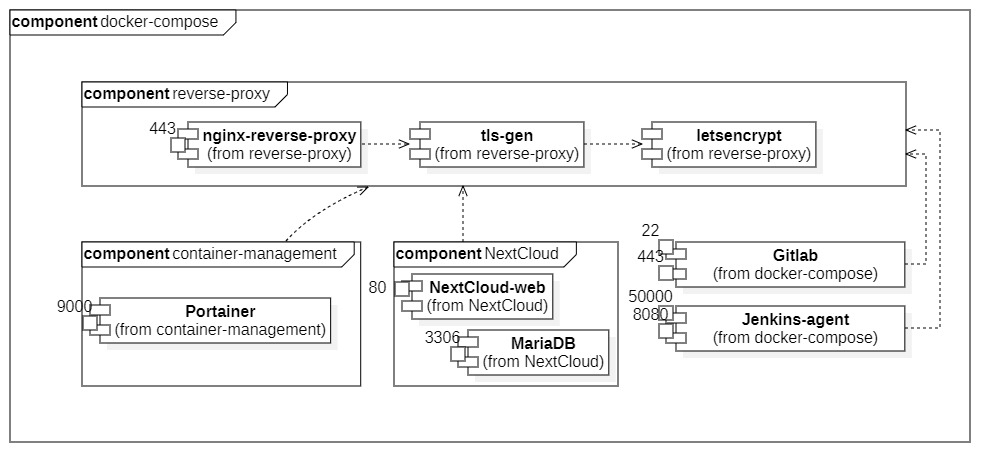
\includegraphics[width=0.8\textwidth,angle=00]{assets/f9.jpg}
\caption{PaaS infrastructure}
\label{fig:f9}
\end{figure}

\section{Application overview and SCM structuring.}

\paragraph{}
Two main applications were in development during this project. We have recommended a better source code management strategy that resulted in separating services into different repos in order to optimize the container image creation process. The resulting deployment diagram Is as follows:
 
\section*{Conclusion}
\paragraph{}In this chapter we have successfully performed



% Introduction
% In this chapter, our analysis is aimed at identifying the key actors in our design, the functional and non-functional needs our system is to provide for. We will then move on to an overview of the sprint bursts we have realized. Finally, we will provide a dissection of the ecosystem in the form of various UML diagrams.
% \section{Capturing requirements}
% \subsection{Identifying key actors}
% In this context, an actor is a user or any other system that interacts with the subject by exchanging signals and data.
% \subsubsection*{Cloud architecture related actors:}
% In order to have a devSecOPS compliant approach, it needs to be built on top of a containerized, highly available cloud infrastructure:
% \newline
% -	Cloud architect: He is responsible for designing and implementing cloud computing solutions.
% \newline
% -	IaC tools: Although being a piece of software, it is necessary in order to automate provisioning and configuration of resources.
% \newline
% -	Cloud provider: Usually a third-party entity that allows for elastically allocating resources.
% \newline
% -	DevSecOPS team: A devSecOPS engineer is the consumer in this case, he uses the provisioned resources to build an ecosystem that is compliant with organizational needs.
% \subsubsection*{CI/CD related actors:}
% The cloud resources hold the value of a tool that is then leveraged to assist the development process:
% \newline
% -	DevSecOPS team: uses the provisioned resources and follows an agile devSecOPS approach to build an ecosystem that is compliant with organizational needs.
% \newline
% -	Developer: A consumer of the devSecOPS ecosystem as well as the CI/CD workflow.
% \newline
% -	Company client: He is the end user and provides the specifications on software development.

% \subsection{Functional requirements}

% Formulating an understanding on functional requirements is a primordial phase in the implementation of the subject.
% \newline
% -	A cloud-based infrastructure capable of hosting the devSecOPS ecosystem in terms of compute resources, storage and networking.
% \newline
% -	A continuous integration platform : The desired goal is to provide a CI workflow that channels the development effort in order to continuously ensure code quality.
% \newline
% -	A CD workflow: provide an automated and continuous delivery and deployment process.

% \subsection{Non-functional requirements}
% -	High availability and resilience: Typically satisfied by distributed backend resources, orchestration and load balancing of workloads. \newline
% -	Performance and scalability: Usually dependent on the cloud provider as well as the used technologies.\newline
% -	Security: An inbuilt quality that cloud and DevSecOPS offer by design.\newline
% -	Observability: A highly achievable need due the pluggability of containerized environments.\newline
% -	Usability: A somewhat hard to achieve requirement due to the rarity of a technologically adept workforce. \newline
% -	Relatively low cost : the need to prioritize self-hosting and adopting opensource alternatives.

% \newpage
% \section{Product backlog }

% \subsection{Backlog history }

% \begin{longtable}[!ht]{|m{1cm}|m{3cm}|m{1cm}|m{7cm}|m{1.2cm}|}
% \hline
%  {\textbf{Epic ID}} & {\textbf{EPIC}} & {\textbf{Story ID}} & {\textbf{Story}} & {\textbf{Prior-ity}} \\
%  \hline
% 0 & \raggedright Certified devSecOps training &	0.1 &	Managing and running custom VMs. & \\
% \cline{3-5}
% &   & 0.2 &	Managing docker containers.	& \\
% \cline{3-5}
% &   & 0.3 &	CI/CD pipelines. & \\
% \hline
% 1 & Maintenance and cleanup. &	1.1	& Exploring existing infrastructure and resources. & \\
% \cline{3-5}
% &   &	1.2 & Performing maintenance on enterprise assets. & \\

% \hline
% 2 & Cloud design &	2.1 &	Information gathering phase. & \\
% \hline
% 3 & Resource provisioning &	3.1 &	Provisioning resources using IaC playbooks. & \\
% \hline
% 4 & Infrastructure setup. &	4.1 &	Infrastructure setup using IaC playbooks. & \\
% \hline
% 5 & \raggedright Initial PaaS setup. &	5.1 &	Setting up ingress controller and TLS certificate provisioner.	 & \\
% \cline{3-5}
% &   & 5.2 &	Setting distributed storage backend.	 & \\
% \cline{3-5}
% &   & 5.3 &	Setting up network load balancer.	 & \\
%   \hline
% 6 & Deployment of CI/CD platform &	6.1 &	Setting up personalized CI/CD orchestrator.	 & \\
% \cline{3-5}
% &   & 6.2 &	Setting up quality gate (CI).	 & \\
% \cline{3-5}
% &   & 6.3 & Setting up CD controller.	 & \\
%   \hline
% 7 & \raggedright Preparation of automated CICD workflows. &	7.2 &	Structuring SCM backend	 & \\
% \cline{3-5}
% &   & 7.2 &	 \raggedright Using GitOPS and devOPS tools to automate CI/CD pipelines.	 & \\
%    \hline
%    \newpage
%      \hline
% 8 & \raggedright Deployment of authentication / authorization backend 	& 8.1 & \raggedright Self-managing distributed database storage backends (redis, mongoDB, postgresql).	 & \\
% \cline{3-5}
% &   & 8.2 &	\raggedright Deployment and configuration of authentication and authorization services.	 & \\
% \cline{3-5}
% &   & 8.3 &	\raggedright Configuring forward auth middlewares for secure access.	 & \\
%    \hline
% 9 & \raggedright Implement a resilient disaster recovery strategy. & 9.1 &\raggedright  Provisioning cloud storage resources.		 & \\
% \cline{3-5}
% &   & 9.2 & \raggedright Preparing and applying backup strategy for application specific data.	 & \\
% \cline{3-5}
% &   & 9.3 &	\raggedright Preparing and applying backup strategy for PaaS specific workloads.	 & \\
%  \hline
% 10	& \raggedright Load testing, benchmarking.& 10.1 & Load testing and benchmarking of assets. & \\	
% \hline

% \end{longtable}
% % \raggedright for space issue

% \newpage
% \subsection{Sprint planification }
% The project lasted seven months and a half starting in March, 1st 2022. Overall ten sprints have been followed with the typical duration of 3 weeks for each. 


% \begin{table}[h!]
% \center
% \begin{tabular}[b]{|m{3cm}|m{8cm}|m{2cm}|}
% \hline
%  {\textbf{Sprint ID}} & {\textbf{Sprint Details }} & {\textbf{Duration }} \\ \hline 
% 0 
% &
% The first period was spent following a company sponsored devSecOps training. The following elements have been covered: 
% Creating vm images using packer, spinning up virtual machines using vagrant,  
% Using docker, docker compose plugin and docker container orchestration in swarm, 
% An overview on CI/CD pipelines using Jenkins. 
% &
% 4 weeks  \\
% \hline
% 1 
% &
% The following two weeks were dedicated to exploring the existing infrastructure. Performing some maintenance and planning for migration. 
% &
% 3 weeks  \\ \hline
% 2 
% &
% Next, we have started the information gathering phase in which we have formed an initial overview of the desired goals we would like to reach. 
% &
% 2 weeks \\ \hline
% 3 
% &
% The use of IaC allowed us to provision the main cloud resources dedicated to hosting the PaaS infrastructure. 
% &
% 2 weeks \\ \hline
% 4 
% &
% An initial setup of the provisioned resources was then automated and performed. 
% &
% 3 weeks \\ \hline
% 5 
% &
% Putting in place the basic PaaS services, namely a distributed storage backend, a layer 2 load balancer, a cloud-native layer 4 ingress controller to route requests serving also as a reverse proxy and an application load balancer. 
% &
% 3 weeks \\ \hline
% 6 
% &
% Mounting the backing CI/CD services which are mostly personalized to company needs. 
% &
% 3 weeks \\ \hline
% 7 
% &
% Levering the CI/CD ecosystem to put in place pipelines to automate product testing, code quality checks, and delivery. 
% &
% 4 weeks \\ \hline
% 8 
% &
% Securing access to company assets using an Authentication/Authorization middleware. 
% &
% 3 weeks \\ \hline
% 9 
% &
% Putting in place a disaster recovery strategy that leverages distributed storage and S3 compliant object storage. 
% &
% 3 weeks \\ \hline
% 10 
% &
% Assessing the performance of the PaaS put in place and planning to enhancements 
% &
% 2 weeks \\ \hline
% \end{tabular}
% \caption{Table Sprint planification}
% \textcolor{white}{I} \label{tab:tab-m}
% \end{table}

% \section{Modeling for cloud architecture and devops }
% \subsection{Class diagram for cloud architecture }

% \subsection{Technological choices }
% \subsubsection*{Development tools }

% \newpage
% \subsubsection*{Infrastructure as code tools  }

% \subsubsection*{Containerization and orchestration techniques  }
% \subsubsection*{Self-hosted paas services }
% \subsubsection*{Cloud provider choice}


% \section*{Conclusion}
